\let\negmedspace\undefined
\let\negthickspace\undefined
\documentclass[journal,12pt,onecolumn]{IEEEtran}
\usepackage{cite}
\usepackage{amsmath,amssymb,amsfonts,amsthm}
\usepackage{algorithmic}
\usepackage{graphicx}
\usepackage{textcomp}
\usepackage{xcolor}
\usepackage{txfonts}
\usepackage{listings}
\usepackage{enumitem}
\usepackage{mathtools}
\usepackage{gensymb}
\usepackage{comment}
\usepackage[breaklinks=true]{hyperref}
\usepackage{tkz-euclide} 
\usepackage{listings}
\usepackage{gvv}                                        
%\def\inputGnumericTable{}                                 
\usepackage[latin1]{inputenc}                                
\usepackage{color}                                            
\usepackage{array}                                            
\usepackage{longtable}                                       
\usepackage{calc}   
\usepackage{multicol}
\usepackage{multirow}                                         
\usepackage{hhline}                                           
\usepackage{ifthen}                                           
\usepackage{lscape}
\usepackage{tabularx}
\usepackage{array}
\usepackage{float}
\usepackage{circuitikz}

\newtheorem{theorem}{Theorem}[section]
\newtheorem{problem}{Problem}
\newtheorem{proposition}{Proposition}[section]
\newtheorem{lemma}{Lemma}[section]
\newtheorem{corollary}[theorem]{Corollary}
\newtheorem{example}{Example}[section]
\newtheorem{definition}[problem]{Definition}
\newcommand{\BEQA}{\begin{eqnarray}}
\newcommand{\nCr}[2]{\,^{#1}C_{#2}}
\newcommand{\EEQA}{\end{eqnarray}}

\begin{document}
\vspace{3cm}
\title{DIGITAL THERMOMETER USING PT-100}
\author{Harsha B J and Bhargav K}
\maketitle

\newpage
\tableofcontents

\newpage
\bigskip

\section{\textbf{Objective}}
The objective of this project is to design and implement a digital thermometer that measures the temperature using a PT-100 Resistance Temperature Detector (RTD), processes the signal through an Arduino microcontroller, and displays the temperature on a 16$\times$2 LCD. In this experiment, the relationship between the voltage across
the PT-100 and the temperature is determined using linear regression (least squares
method).

\section{\textbf{Training Data}}
The training data gathered by the PT-100 to train the Arduino is shown in Table
\ref{tab:train}.

\begin{table}[H]
    \centering
    % This is a LaTeX table.
\documentclass{article}
% You can include this in your main .tex document using % This is a LaTeX table.
\documentclass{article}
% You can include this in your main .tex document using % This is a LaTeX table.
\documentclass{article}
% You can include this in your main .tex document using \input{training_data.tex}
% Or copy the \begin{table}...\end{table} block into your document.

\begin{document}
% This is a LaTeX table with full grid lines.
% You'll need the \usepackage{array} package in your preamble for the formatting.

% This is a LaTeX table with full grid lines.
% You'll need the \usepackage{array} package in your preamble for the formatting.

\begin{table}[h]
\centering
\caption{Training Data}
\label{tab:training_data}
\begin{tabular}{|c|c|}
\hline
\textbf{Temperature ($^{\circ}$C)} & \textbf{Voltage (V)} \\
\hline
25.1 & 2.15543 \\
\hline
25.9 & 2.16031 \\
\hline
34.5 & 2.19941 \\
\hline
36.1 & 2.20430 \\
\hline
40.0 & 2.21408 \\
\hline
46.3 & 2.24340 \\
\hline
51.1 & 2.26295 \\
\hline
53.1 & 2.26784 \\
\hline
59.1 & 2.29228 \\
\hline
62.9 & 2.30694 \\
\hline
68.2 & 2.32649 \\
\hline
74.8 & 2.35093 \\
\hline
80.4 & 2.37048 \\
\hline
89.0 & 2.39980 \\
\hline
90.3 & 2.40469 \\
\hline
92.0 & 2.40958 \\
\hline
95.8 & 2.42424 \\
\hline
97.3 & 2.42913 \\
\hline
\end{tabular}
\end{table}
\end{document}
% Or copy the \begin{table}...\end{table} block into your document.

\begin{document}
% This is a LaTeX table with full grid lines.
% You'll need the \usepackage{array} package in your preamble for the formatting.

% This is a LaTeX table with full grid lines.
% You'll need the \usepackage{array} package in your preamble for the formatting.

\begin{table}[h]
\centering
\caption{Training Data}
\label{tab:training_data}
\begin{tabular}{|c|c|}
\hline
\textbf{Temperature ($^{\circ}$C)} & \textbf{Voltage (V)} \\
\hline
25.1 & 2.15543 \\
\hline
25.9 & 2.16031 \\
\hline
34.5 & 2.19941 \\
\hline
36.1 & 2.20430 \\
\hline
40.0 & 2.21408 \\
\hline
46.3 & 2.24340 \\
\hline
51.1 & 2.26295 \\
\hline
53.1 & 2.26784 \\
\hline
59.1 & 2.29228 \\
\hline
62.9 & 2.30694 \\
\hline
68.2 & 2.32649 \\
\hline
74.8 & 2.35093 \\
\hline
80.4 & 2.37048 \\
\hline
89.0 & 2.39980 \\
\hline
90.3 & 2.40469 \\
\hline
92.0 & 2.40958 \\
\hline
95.8 & 2.42424 \\
\hline
97.3 & 2.42913 \\
\hline
\end{tabular}
\end{table}
\end{document}
% Or copy the \begin{table}...\end{table} block into your document.

\begin{document}
% This is a LaTeX table with full grid lines.
% You'll need the \usepackage{array} package in your preamble for the formatting.

% This is a LaTeX table with full grid lines.
% You'll need the \usepackage{array} package in your preamble for the formatting.

\begin{table}[h]
\centering
\caption{Training Data}
\label{tab:training_data}
\begin{tabular}{|c|c|}
\hline
\textbf{Temperature ($^{\circ}$C)} & \textbf{Voltage (V)} \\
\hline
25.1 & 2.15543 \\
\hline
25.9 & 2.16031 \\
\hline
34.5 & 2.19941 \\
\hline
36.1 & 2.20430 \\
\hline
40.0 & 2.21408 \\
\hline
46.3 & 2.24340 \\
\hline
51.1 & 2.26295 \\
\hline
53.1 & 2.26784 \\
\hline
59.1 & 2.29228 \\
\hline
62.9 & 2.30694 \\
\hline
68.2 & 2.32649 \\
\hline
74.8 & 2.35093 \\
\hline
80.4 & 2.37048 \\
\hline
89.0 & 2.39980 \\
\hline
90.3 & 2.40469 \\
\hline
92.0 & 2.40958 \\
\hline
95.8 & 2.42424 \\
\hline
97.3 & 2.42913 \\
\hline
\end{tabular}
\end{table}
\end{document}
    \caption{Training data.}
    \label{tab:train}
\end{table}

The C++ source \texttt{codes/data.cpp} was used along with \textit{platformio} to drive the Arduino.

The approximation is shown in Fig. \ref{fig:train}.
\begin{figure}[H]
    \centering
    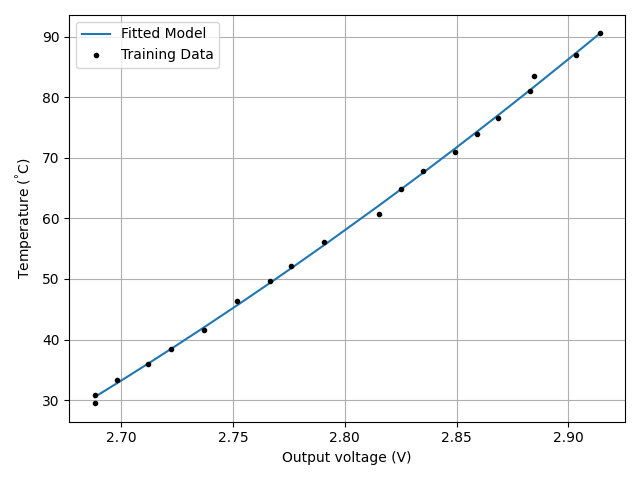
\includegraphics[width=0.6\columnwidth]{figs/temp_vs_voltage/train.png}
    \label{fig:train}
\end{figure}

\vspace{2cm}

\section{\textbf{Theory}}
The PT-100 sensor changes resistance with temperature. Its nominal resistance is 100 $\ohm$
at 0 $\degree$C, and the resistance increases approximately linearly with temperature:
\begin{align}
R_T = R_o(1 + \alpha T)
\end{align}
where $\alpha$ = 0.00385 $\degree C^{-1}$. When placed in a Wheatstone bridge circuit, the resistance variation produces a corresponding voltage change, which can be measured and used to infer the temperature.


\section{\textbf{Linear Regression Model}}
To obtain an empirical model relating the measured voltage V to temperature T, we collect calibration data by measuring both quantities over a range of known temperatures. Let the measured data points be ($T_i$ , $V_i$), i = 1, 2,. . , n. We assume a quadratic model for the voltage-temperature relationship
\begin{align}
    V(T) &= n_0+n_1T+n_2T^2 \\
\end{align}
\begin{align}
    \implies \vec{C} = \vec{X^T}\vec{n}  \label{eq:model}
\end{align}
where
\begin{align}
    \vec{n}=\myvec{n_0 \\ n_1 \\ n_2}, 
   \vec{X^T} = \myvec{1 & T_1 & T_1^2 \\ 1 & T_2 & T_2^2 \\ . & . & .\\ . & . & .\\ . & . & . \\ 1 & T_n & T_n^2}, \vec{C} = \myvec{V_1 \\ V_2 \\ . \\ . \\ . \\ V_n}
    \label{eq:x-y-theta-def}
\end{align}



\section{\textbf{Solution}}
We approximate $\vec{n^T} = \myvec{n_0 & n_1 & n_2}$ using the least squares method. Using the pseudo-inverse method, the solution to \eqref{eq:model} is
\begin{align}
    \vec{n} = \brak{\vec{XX}^\top}^{-1}\vec{X}\vec{C}
\end{align}
The Python code \texttt{codes/main.py} solves for $\vec{n}$.
The calculated value of $\vec{n}$ is
\begin{align}
    \vec{n} = \myvec{2.54834\\4.8818\times10^{-3}\\-9.370283\times10^{-6}}
    \label{eq:opt-theta-1}
\end{align}
To obtain temperature as a function of measured voltage (for Arduino implementation), we rearrange or numerically invert the above relation:
\begin{align}
T(V) = a_0 + a_1V + a_2V^2
\end{align}
The coefficients $a_i$ can again be found by applying the least squares method to the ($V_i$, $T_i$)
data, which yields
\begin{align}
    \vec{n} = \myvec{666.3569\\-699.7908329\\172.33050} = \myvec{a_0 \\ a_1 \\ a_2}
    \label{eq:opt-theta-2}
\end{align}


\section{\textbf{Validation}}
The validation data set is shown in Table \ref{tab:valid}. The results of the
validation are shown in Fig. \ref{fig:valid}.
\begin{table}[H]
    \centering
    \documentclass[journal,12pt,onecolumn]{IEEEtran}
\author{EE25BTECH11025\_EE25BTECH11023}

\begin{document}

\maketitle
\begin{center}
Validation Data\\
\vspace{0.3cm}
\begin{tabular}{|c|c|}
\hline
Temperature($C^o$)&Voltage(V)\\
\hline
90.6&2.400\\
\hline
76.5&2.351\\
\hline
62.2&2.297\\
\hline
43.6&2.229\\
\hline
\end{tabular}
\end{center}

\end{document}




    \caption{Validation data.}
    \label{tab:valid}
\end{table}
\begin{figure}[H]
    \centering
    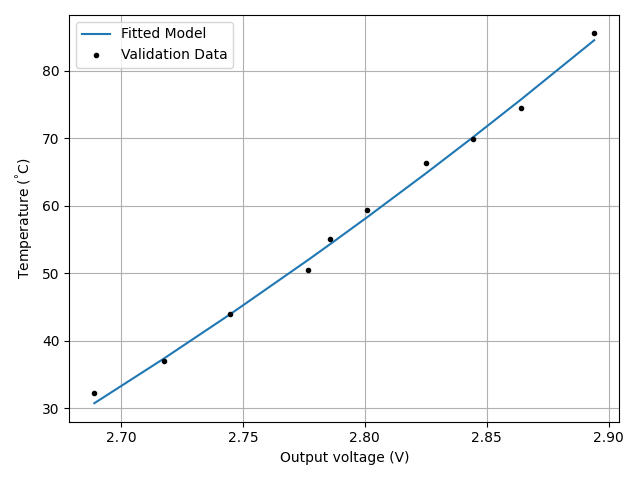
\includegraphics[width=0.6\columnwidth]{figs/temp_vs_voltage/valid.png}
    \label{fig:valid}
\end{figure}

\section{\textbf{Conceptual logic implemented in the code}}
The provided program implements a quadratic regression model to establish the relationship between temperature and output voltage. It begins by loading the training data consisting of temperature (in $\degree$C) and voltage (in V) readings. A design matrix is then constructed using three terms: a constant, the temperature, and the square of the temperature. By applying the least squares method, the program determines the model coefficients that best fit the data. This fitted model is then used to generate predicted voltage values, which are plotted against the actual training data to visualize the accuracy of the fit.\\
\\
Subsequently, the program loads a separate validation dataset to evaluate the performance of the derived model on unseen data. The fitted curve and the actual validation data points are plotted together, allowing a clear comparison of the predicted and measured values. The resulting plots are saved for documentation, and the computed model parameters are printed for further analysis. In essence, the code effectively demonstrates the use of polynomial regression for sensor calibration and performance verification.

\section{\textbf{Observation}}
The observations made while conducting the experiment are as follows,
\begin{enumerate}
    \item The readings of arduino had an offset of a few millivolts for every cycle of reading.
    Solution: We wrote an algorithm to take an average of a few sample readings and computed the temperature using it which gave a good precision.
    \item The values of the temperature had an offset of $\pm \,3\degree$ celcius due to the hardware \\malfunctioning.
    \item the accuracy of the training model and validation data is close enough with a less validation.
\end{enumerate}


\section{\textbf{Circuit Diagram}}
\begin{figure}[H]
    \centering
    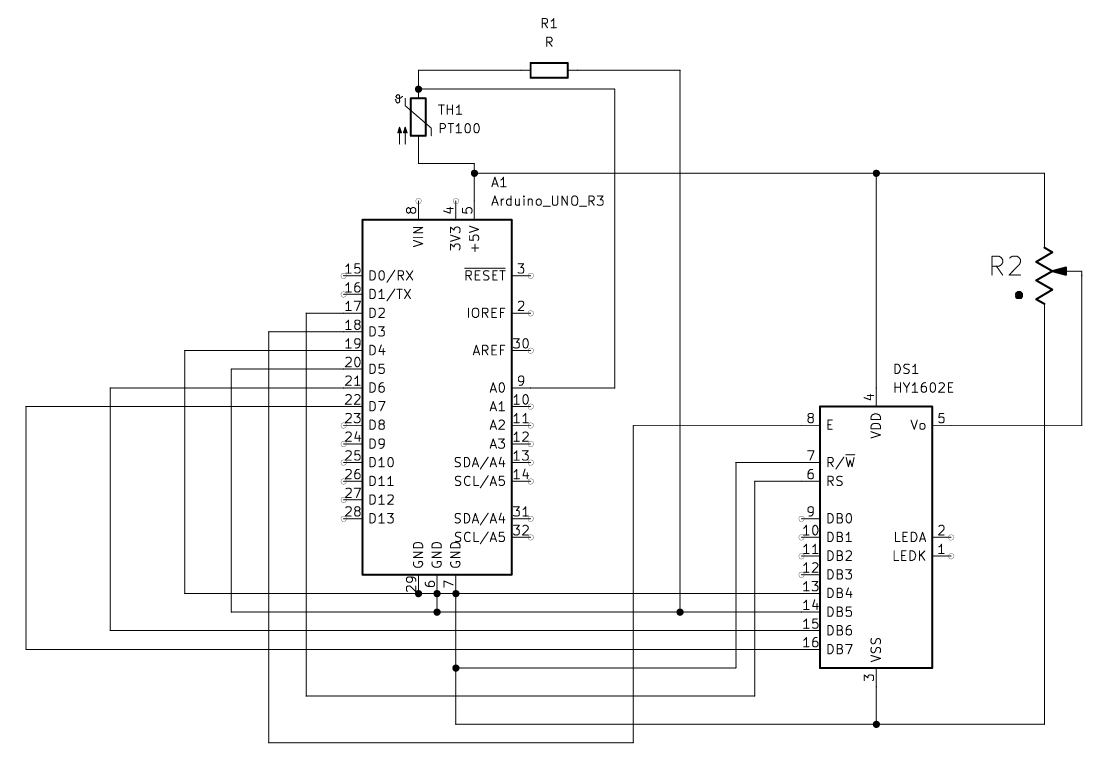
\includegraphics[width=0.8\columnwidth]{figs/circuit diagram.jpeg}
    \label{fig:crtdiagram}
\end{figure}



\section{\textbf{Conclusion}}

This project used Python for machine learning to calibrate the temperature sensor with linear regression. Arduino collected sensor data and showed real-time results. Python made the analysis easier and more accurate, while Arduino handled the hardware side. This simple combination of Python and Arduino creates a smart, affordable device by merging data science and embedded systems effectively.


\end{document}
